\section{The Geometry of Euclidean Space}
\subsection{$n$-Dimensional Euclidean Space}
Let $\R^n$ be the vector space of $n$-tuples $\mathbf{x}=\left(x_1, x_2, \ldots, x_n\right)$ with entries from $\R$, defined under the operations of coordinate-wise addition and multiplication. For $\mathbf{x}, \mathbf{y} \in \R^n$ and $c \in \R$, we have that,
\begin{align*}
    &\mathbf{x} + \mathbf{y} = (x_1 + y_1, \ldots, x_n + y_n) \\
    &c \mathbf{x} = \left(c x_1, c x_2, \ldots, c x_n\right)
\end{align*}
We will consider the Euclidean inner product on $\R^n$ defined by,
\begin{align*}
    &\langle\mathbf{x}, \mathbf{y}\rangle \longmapsto \mathbf{x} \cdot \mathbf{y} \\
    &\mathbf{x} \cdot \mathbf{y} := \sum_{i=1}^n x_i \cdot y_i
\end{align*}
For $\mathbf{x} \in \R^n$, we define the norm of $\mathbf{x}$ to be,
\[\|x\| = \sqrt{\langle \mathbf{x}, \mathbf{x}\rangle} =  \sqrt{\mathbf{x} \cdot \mathbf{x}}\]
The Euclidean distance between $\mathbf{x}, \mathbf{y} \in \R^n$ is defined as,
\[d(\mathbf{x}, \mathbf{y}) = \|x - y\| =\sqrt{\sum_{i=1}^n\left(x_i-y_i\right)^2}\]

\begin{marginfigure}
The geometric significance of the norm $\|\cdot\|$ in $\R^2$ is shown below. Recall that,
\[\cos \theta = \frac{\mathbf{x} \cdot \mathbf{y}}{\|\mathbf{x}\|\|\mathbf{y}\|}\]
\begin{center}
       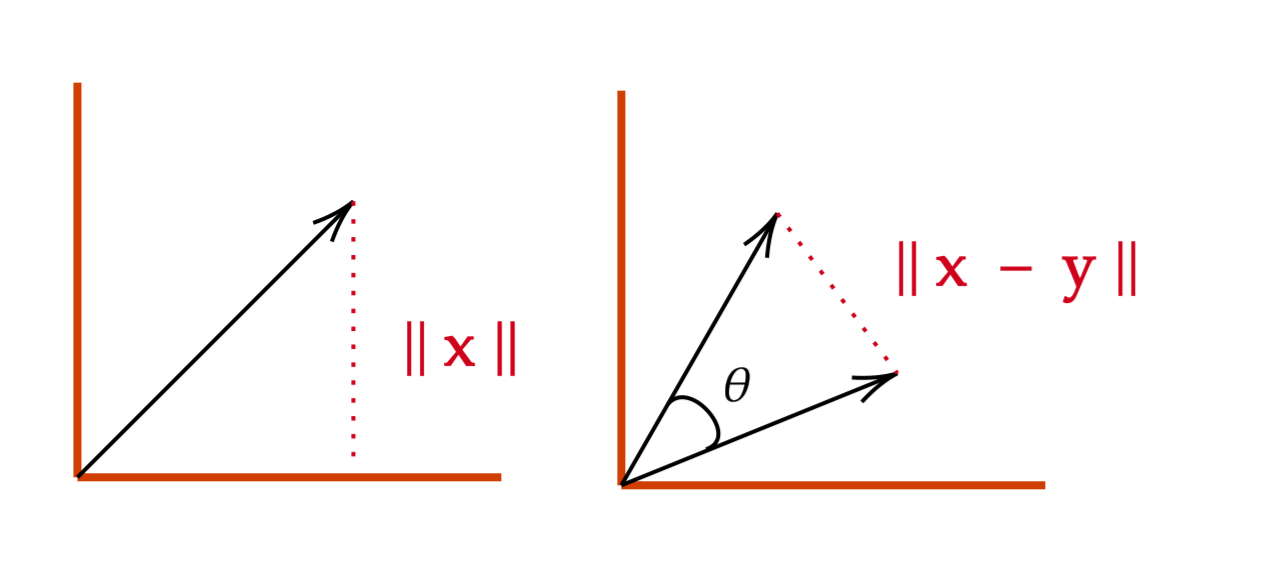
\includegraphics[width=\textwidth]{figures/wk-1/fig-1.png}
\end{center}
\end{marginfigure}

\begin{rmk}
    For $\mathbf{x}, \mathbf{y}, \mathbf{z} \in \R^n$ and $\alpha, \beta \in \R$, we have,
    \begin{enumerate}
        \item $(\alpha \mathbf{x}+\beta \mathbf{y}) \cdot \mathbf{z}=\alpha(\mathbf{x} \cdot \mathbf{z})+\beta(\mathbf{y} \cdot \mathbf{z})$
        \item $\mathbf{x} \cdot \mathbf{y}=\mathbf{y} \cdot \mathbf{x}$
        \item $\mathbf{x} \cdot \mathbf{x} \geq 0$
        \item $\mathbf{x} \cdot \mathbf{x}=0$ if and only if $\mathbf{x}=\mathbf{0}$
    \end{enumerate}
\end{rmk}

\begin{thm}[Cauchy-Schwartz Inequality]
     Let $\mathbf{x}, \mathbf{y} \in \R^n$. Then,
     \[|\mathbf{x} \cdot \mathbf{y}|  \leq\|\mathbf{x}\| \cdot \|\mathbf{y}\|\]
\end{thm}

\begin{proof}
     Let $\mathbf{x}, \mathbf{y} \in \R^n$ and $\lambda \in \R^+$. If either $\mathbf{x} = \mathbf{0}$ or $\mathbf{y} = \mathbf{0}$, then the statement holds trivially. Assume that this is not the case. Then,
     \begin{align*}
        p(\lambda) &:= (\mathbf{x}+\lambda \mathbf{y}) \cdot(\mathbf{x}+\lambda \mathbf{y}) \\
        &= \mathbf{x} \cdot \mathbf{x}+ \lambda \cdot \mathbf{y} \cdot \mathbf{x} + \lambda \cdot \mathbf{x} \cdot \mathbf{y} +\lambda^2 (\mathbf{y} \cdot \mathbf{y}) \\
        &= \underbrace{\|\mathbf{x}\|^2}_{c}+ \lambda \cdot \underbrace{2(\mathbf{y} \cdot \mathbf{x})}_{b} +\lambda^2\underbrace{\|\mathbf{y}\|^2}_{a} \geq 0
        \end{align*}
    \sloppy with the second equality holding by the commutativity of the dot product. We have a quadratic polynomial with discriminant,
    \[4(\mathbf{x} \cdot \mathbf{y})-4\|\mathbf{x}\|^2 \cdot\|\mathbf{y}\|^2\]
    which must be non-positive because,
    \[p(\lambda) \geq 0\]
    Simplifying gives that $(\mathbf{x} \cdot \mathbf{y})^2 \leq \|\mathbf{x}\|^2 \cdot\|\mathbf{y}\|^2$ and therefore,
    \[|\mathbf{x} \cdot \mathbf{y}| \leq\|\mathbf{x}\| \cdot \|\mathbf{y}\|\]
\end{proof}

\begin{ex}{Characterizing $p(\lambda)$}{label}
    \begin{center}
       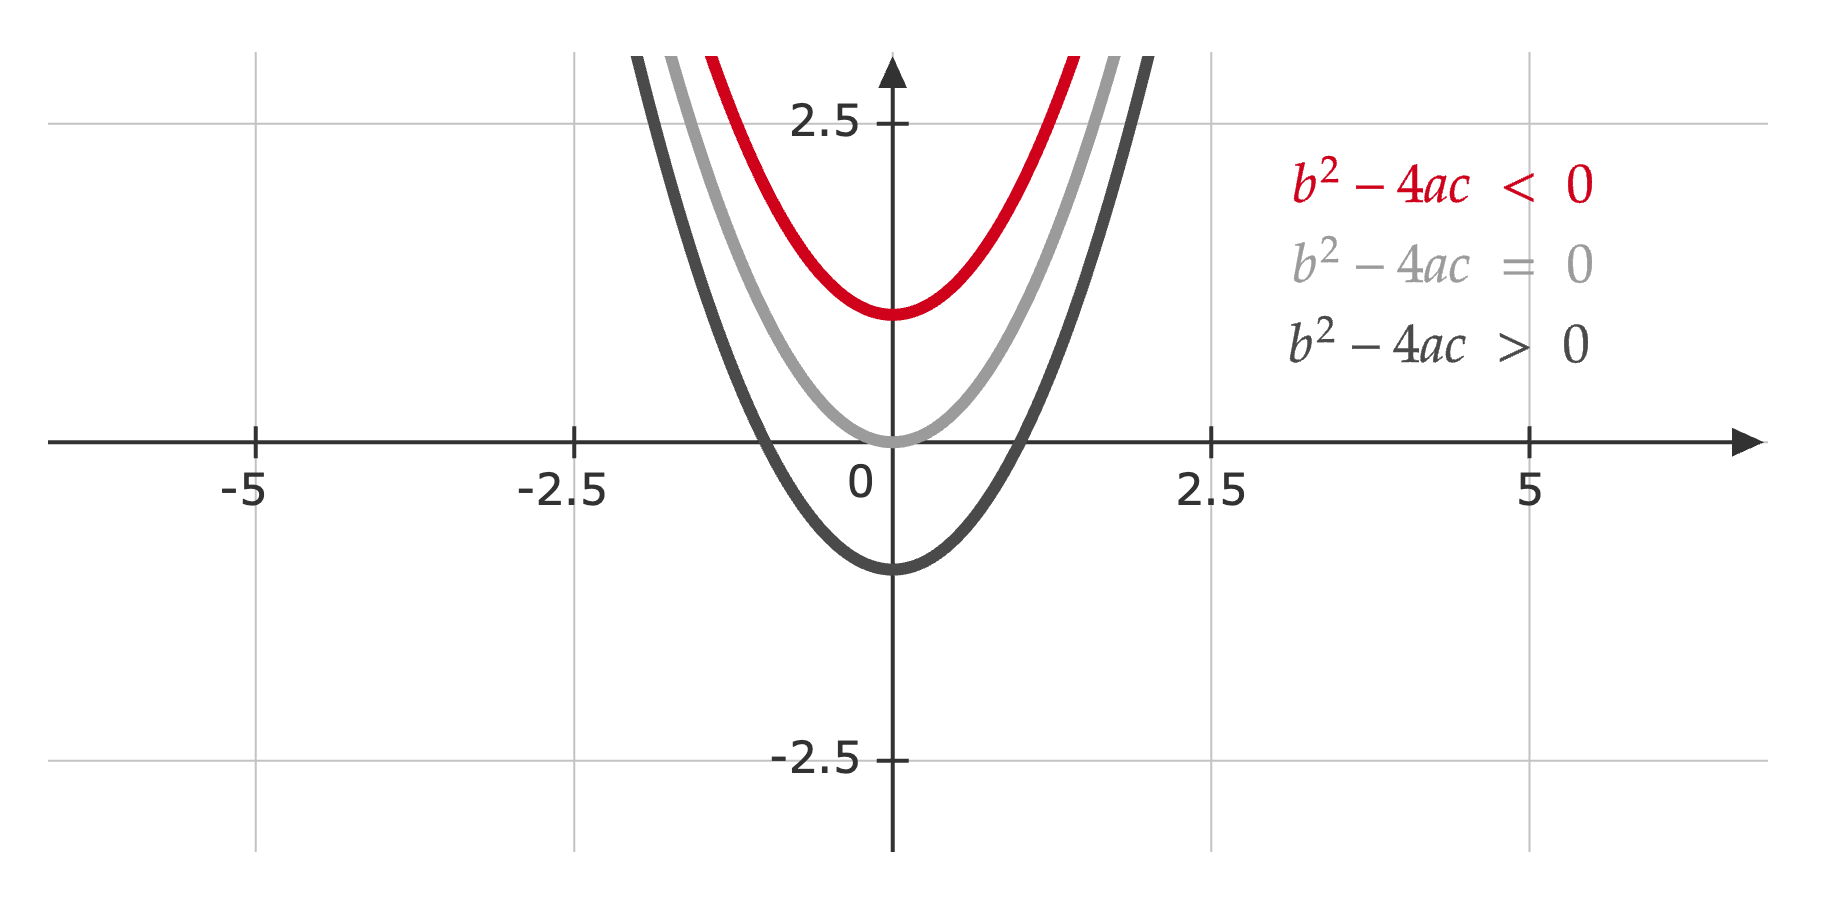
\includegraphics[width=0.8\textwidth]{figures/wk-1/fig-0.png}
    \end{center}
\end{ex}

\begin{cor}[Triangle Inequality]
    Let $\mathbf{x}, \mathbf{y} \in \R^n$. Then,
    \[\|\mathbf{x}+\mathbf{y}\| \leq\|\mathbf{x}\|+\|\mathbf{y}\|\]
\end{cor}

\begin{proof}
     We will consider the case where $\lambda = 1$.
     \begin{align*}
         \|\mathbf{x} + \mathbf{y}\|^2
         &= \|\mathbf{x}\|^2+ 2 |\mathbf{y} \cdot \mathbf{x}| +\lambda^2\|\mathbf{y}\|^2 \\
        &\leq\|\mathbf{x}\|^2+2\|\mathbf{x}\| \cdot\|\mathbf{y}\|+\|\mathbf{y}\|^2 \\
        &=(\|\mathbf{x}\|+\|\mathbf{y}\|)^2
     \end{align*}
     since $|\mathbf{x} \cdot \mathbf{y}|  \leq\|\mathbf{x}\| \cdot \|\mathbf{y}\|$ by Cauchy-Schwartz. This gives that,
     \[\|\mathbf{x} + \mathbf{y}\|^2 \leq (\|\mathbf{x}\|+\|\mathbf{y}\|)^2\]
     which implies the desired result: $\|\mathbf{x}+\mathbf{y}\| \leq\|\mathbf{x}\|+\|\mathbf{y}\|$.
\end{proof}

\begin{marginfigure}
    An orientation is a choice of ordering for our basis $\mathbf{e_1}, \mathbf{e_2}, \mathbf{e_3}$. By convention,
    
    \begin{minipage}{.43\linewidth}
    \begin{align*}
    &\mathbf{e_1} \times \mathbf{e_2}=\mathbf{e_3} \\
    &\mathbf{e_3} \times \mathbf{e_1}=\mathbf{e_2} \\
    &\mathbf{e_2} \times \mathbf{e_3}=\mathbf{e_1}
    \end{align*}
    \end{minipage}
    \begin{minipage}{.43\linewidth}
    \begin{align*}
    &\mathbf{e_1} \times \mathbf{e_1}=0 \\
    &\mathbf{e_2} \times \mathbf{e_2}=0 \\
    &\mathbf{e_3} \times \mathbf{e_3}=0
    \end{align*}
    \end{minipage}
    
    \begin{center}
       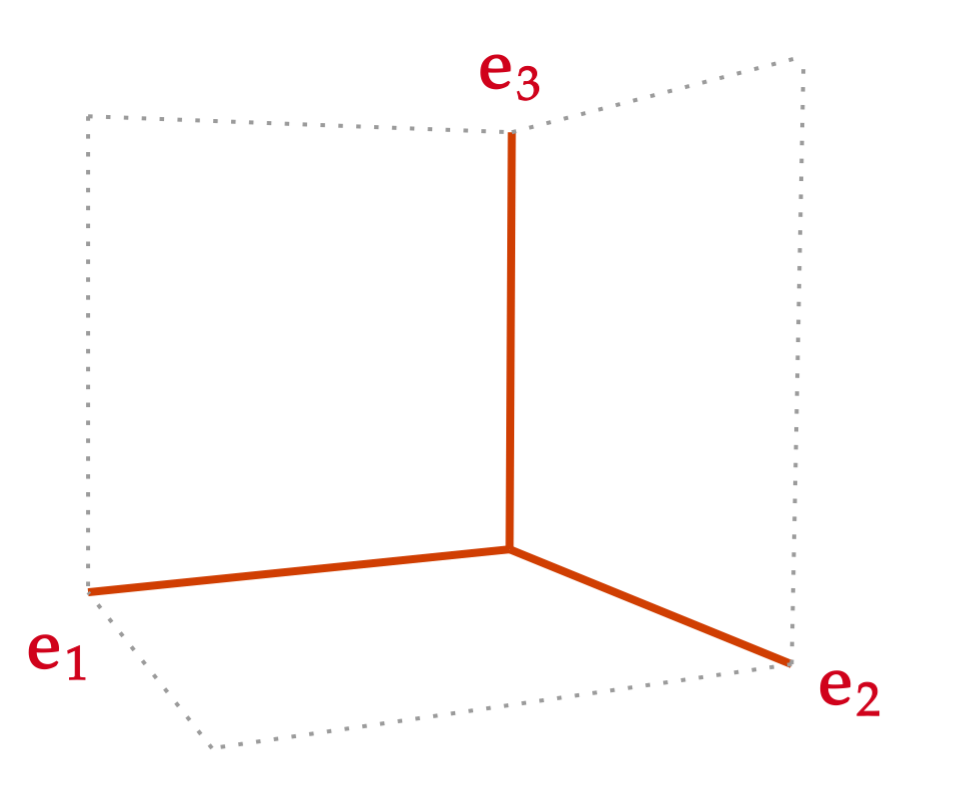
\includegraphics[width=0.8\textwidth]{figures/wk-1/fig-2.png}
    \end{center}
\end{marginfigure}

\newpage 

\subsection{Understanding the Cross Product}
\begin{defn}[Cross-Product]
     Let $\mathbf{e_1}, \mathbf{e_2}, \mathbf{e_3}$ be the standard basis of $\R^3$. The \textbf{cross-product} $\times: \R^3 \times \R^3 \rightarrow \R^3$ is the map defined by,
    \begin{align*}
    \mathbf{x} \times \mathbf{y}
    &=\left|\begin{array}{ccc}
    \mathbf{e_1} & \mathbf{e_2} & \mathbf{e_3} \\
    x_1 & x_2 & x_3 \\
    y_1 & y_2 & y_3
    \end{array}\right|
    \end{align*}
    for two vectors $\mathbf{x}$ and $\mathbf{y}$ in $\R^3$.
\end{defn}

\begin{marginfigure}
    $\mathbf{x} \times \mathbf{y}$ is perpendicular to both $\mathbf{x}$ and $\mathbf{y}$. Moreover, $\|\mathbf{x} \times \mathbf{y}\|$ is the area of the parallelogram spanned by $\mathbf{x}$ and $\mathbf{y}$.
    \begin{center}
           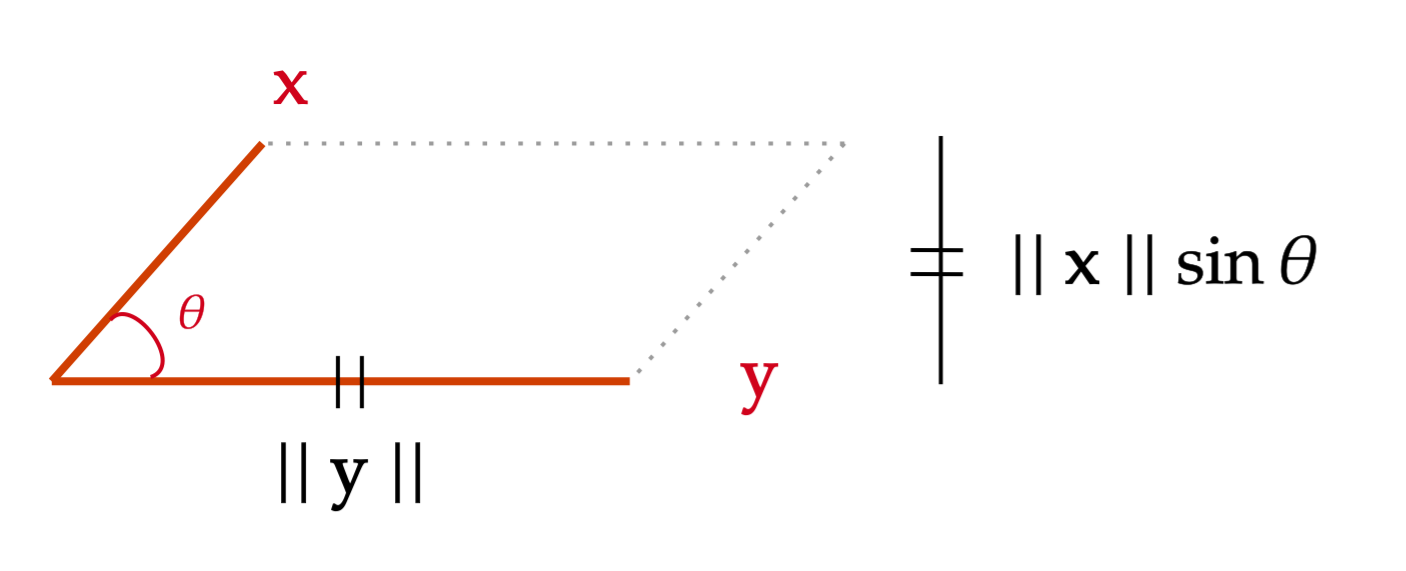
\includegraphics[width=\textwidth]{figures/wk-1/fig-3.png}
    \end{center}
\end{marginfigure}

\begin{rmk}
Let $\mathbf{x}$ and $\mathbf{y}$ be two vectors in $\R^3$. Then,
\[\mathbf{x} \times \mathbf{y}
    =\left(x_1 \mathbf{e_1}+x_2 \mathbf{e_2}+ x_3 \mathbf{e_3}\right) \times \left(y_1 \mathbf{e_1}+y_2 \mathbf{e_2}+y_3 \mathbf{e_3}\right)\]
Expanding and using the fact that,
\begin{align*}
    &\mathbf{e_1} \times \mathbf{e_2} = \mathbf{e_3} \\
    &\mathbf{e_1} \times \mathbf{e_3} = -\mathbf{e_2} \\
    &\mathbf{e_2} \times \mathbf{e_3} = \mathbf{e_1}
\end{align*}
gives the following equality,
\[\mathbf{x} \times \mathbf{y}
    =\mathbf{e_3}\left(x_1 y_2-x_2 y_1\right) -\mathbf{e}_2\left(x_1 y_3-x_3 y_1\right) + \mathbf{e_1}\left(x_2 y_3-x_3 y_2\right)\]
but this is the determinant of the matrix,
\[\left|\begin{array}{ccc}
    \mathbf{e_1} & \mathbf{e_2} & \mathbf{e_3} \\
    x_1 & x_2 & x_3 \\
    y_1 & y_2 & y_3
    \end{array}\right|\]
\end{rmk}

\begin{cor}
   \sloppy  Two vectors $\mathbf{x}, \mathbf{y} \in \R^3$ are linearly independent if and only if their cross-product is non-zero. This result does not hold in higher dimensions because the normal $\mathbf{n}$ satisfying,
    \[\mathbf{x} \times \mathbf{y}=(\|\mathbf{x}\|\|\mathbf{y}\| \sin \Theta) \cdot \mathbf{n}\]
    is no longer unique.
\end{cor}

\subsection{Graphs and Level-Sets}
\begin{marginfigure}
The graph of a function of two variables taking values in $\R$ is,
\begin{center}
       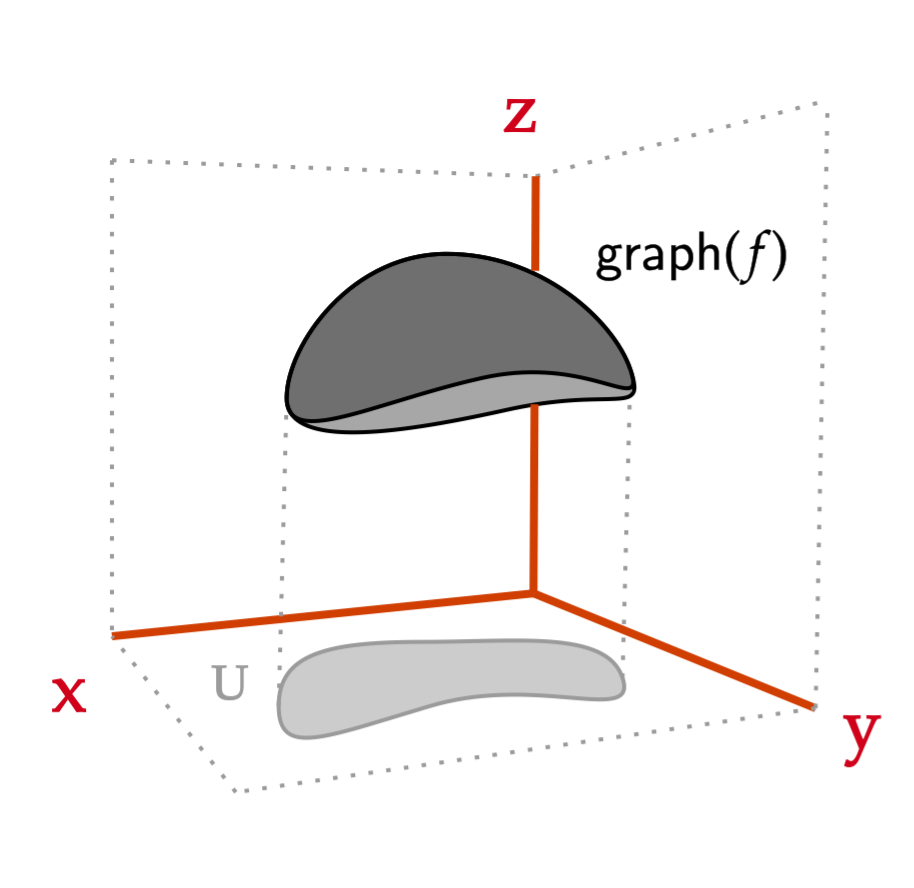
\includegraphics[width=\textwidth]{figures/wk-1/fig-4.png}
\end{center}
\end{marginfigure}

\begin{defn}[Graphs of Functions]
     The \textbf{graph} of a function,
     \[f: U \subseteq \R^n \rightarrow \R\]
     is the subset of $\mathbb{R}^{n+1}$ given by,
     \[\texttt{graph}(f) := \left\{(\mathbf{x}, f(\mathbf{x})) \in \mathbb{R}^{n+1} \mid \mathbf{x} \in U\right\}\]
\end{defn}

\begin{marginfigure}
    The level set is called a \textbf{level curve} if $n = 2$ and a \textbf{level surface} if $n = 3$.
\end{marginfigure}

\begin{defn}[Level Set]
     Let $f: U \subseteq \R^n \rightarrow \R$ and $c \in \R$. The \textbf{level set} of value $c$ is the subset of $\mathbb{R}^{n}$ given by,
     \[\{\mathbf{x} \in U \mid f(\mathbf{x}) = c\} = f^{-1}(\{c\})\]
\end{defn}

\begin{rmk}
    If $c_1, c_2 \in \text{range}(f)$ are such that $c_1 \neq c_2$, then,
    \[f^{-1}(\{c_1\}) \cap f^{-1}(\{c_2\}) = \emptyset\]
\end{rmk}

\subsection{Examples of Graphs in $\R^3$}
\begin{marginfigure}
    \begin{center}
        \textbf{Paraboloid of Revoluation}
        \[f(x, y) = x^2 + y^2\]
        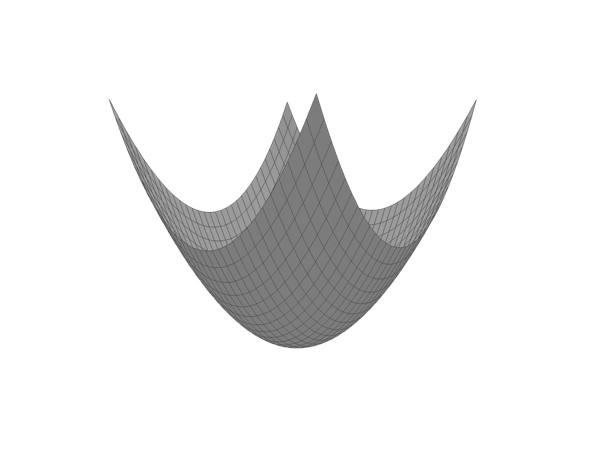
\includegraphics[width=\linewidth]{figures/wk-1/fig-5.png}
        \LineBreak
        \textbf{Paraboloid of Translation}
        \[f(x, y) = x^2 + 1\]
        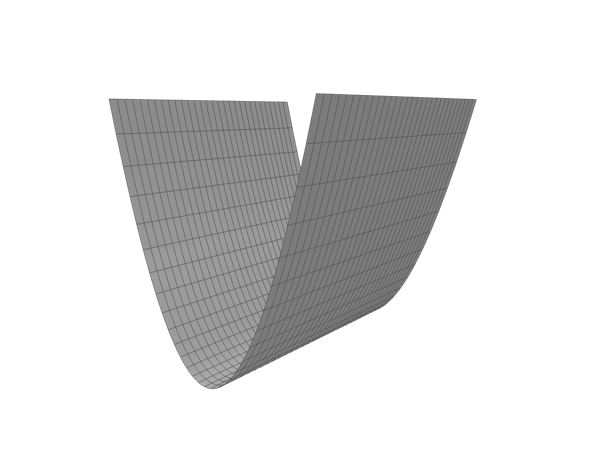
\includegraphics[width=\linewidth]{figures/wk-1/fig-7.png}
        \LineBreak
        \textbf{Lower Hemisphere}
        \[f(x, y) = - \sqrt{1 - (x^2 + y^2)}\]
        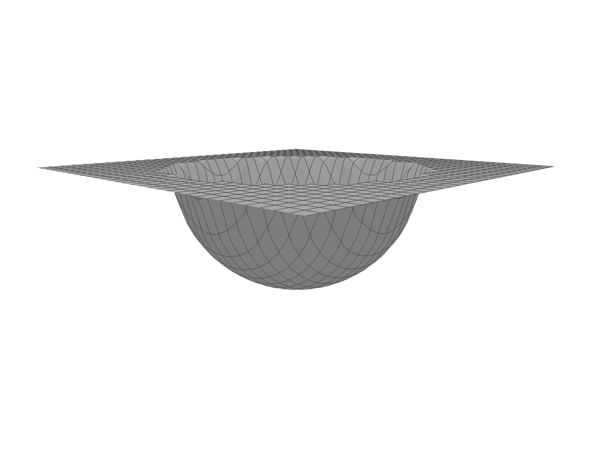
\includegraphics[width=\linewidth]{figures/wk-1/fig-9.png}
    \end{center}
\end{marginfigure}

\begin{ex}{Paraboloid of Revolution}{label}
    The function $f: \R^2 \rightarrow \R$ defined by
    \[f(x, y) = x^2 + y^2\]
    is a \textbf{paraboloid of revolution}. It has range$(f) = [0, \infty)$ and
    \[f^{-1}(\{0\}) = \{(0, 0)\} \text{ and } f^{-1}(\{c\}) \text{ is a circle of radius } \sqrt{c}\]
\end{ex}

\begin{ex}{Paraboloid of Translation}{label}
    The function $f: \R^2 \rightarrow \R$ defined by
    \[f(x, y) = x^2 + 1\]
    is a \textbf{paraboloid of translation}. It has range$(f) = [1, \infty)$ and,
    \[f^{-1}(\{c\}) \text{ is a pair of lines at } \pm \sqrt{c-1}\]
\end{ex}

\begin{ex}{Lower Hemisphere}{label}
    The function $f: \R^2 \rightarrow \R$ defined by
\[f(x, y) = - \sqrt{1 - (x^2 + y^2)}\]
    is a \textbf{lower hemisphere}. It has range$(f) = [-1, 0]$ and,
    \[f^{-1}(\{c\}) \text{ is a circle of radius } \sqrt{1-c^2}\]
\end{ex}

\begin{ex}{Connected Components of the Level Sets}{label}
    Level sets of a single value need not belong to a single connected component. The function $f: \R^2 \rightarrow \R$ defined by
    \[f(x, y) = x y\]
     has range$(f) = (-\infty, \infty)$. Geometrically,
    \begin{center}
        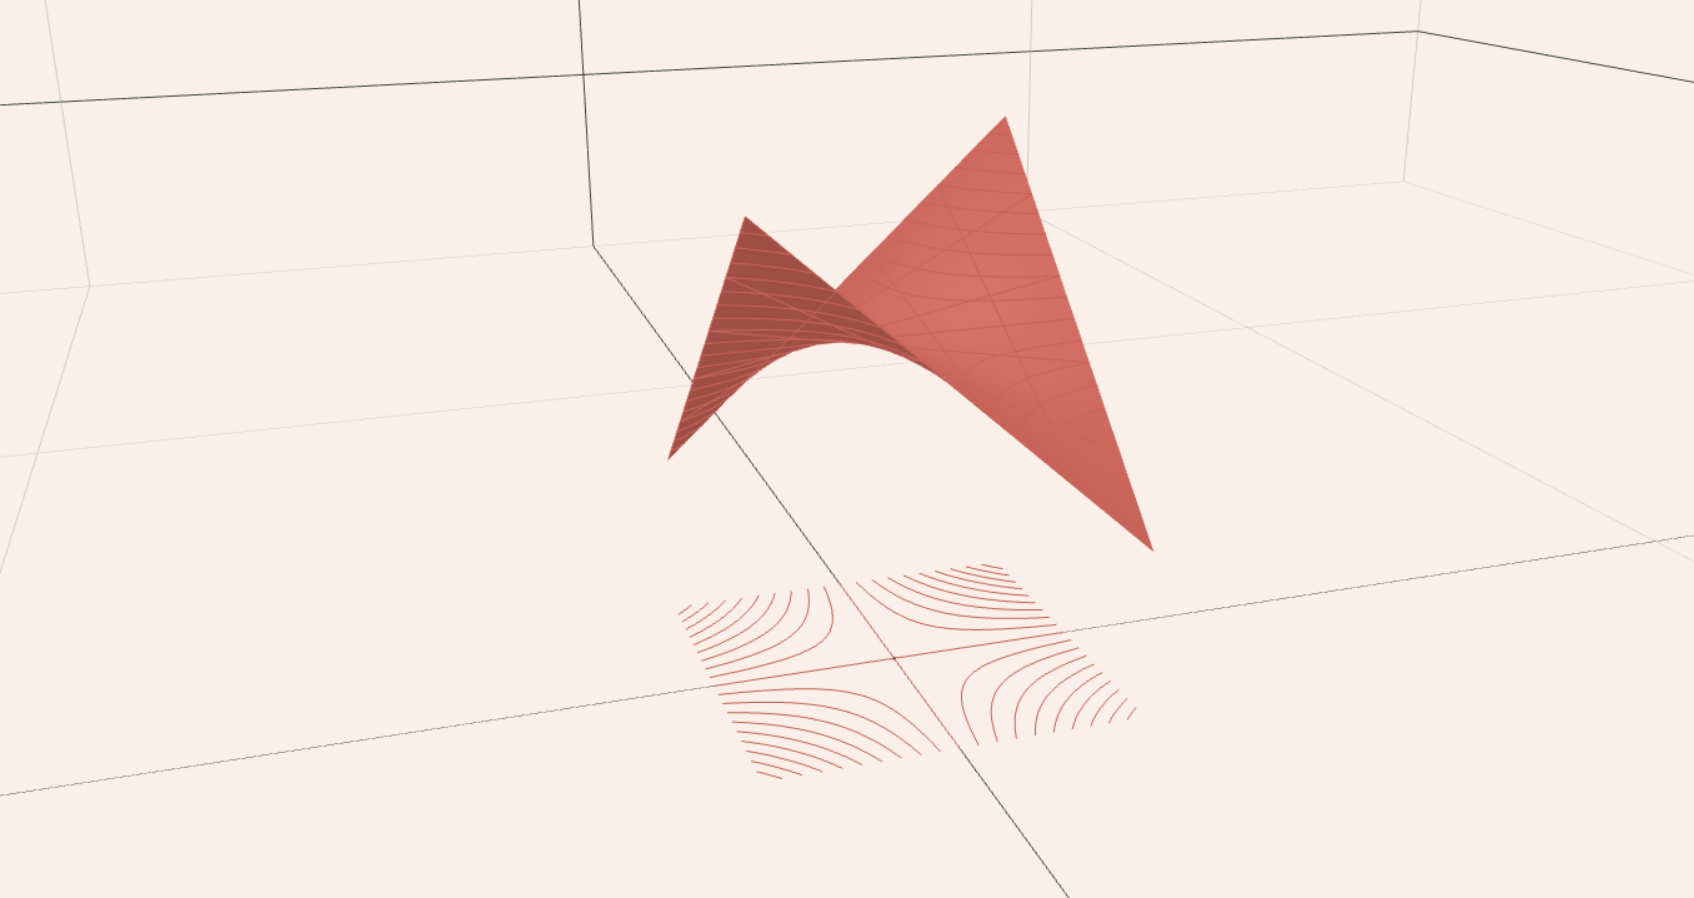
\includegraphics[width=\linewidth]{figures/wk-1/fig-00.png}
    \end{center}
\end{ex}

\begin{marginfigure}
    We can also analyze functions taking values from $\R^3$. For instance,
    \[f(x, y, z) = x + y + z\]
    has range$(f) = \R$ and
    \[f^{-1}(\{c\}) = \{(x, y, z) \mid x + y + z = c\}\]
    is a plane intersecting the $x$-axis at $c$. This can be visualized as follows,
    \begin{center}
        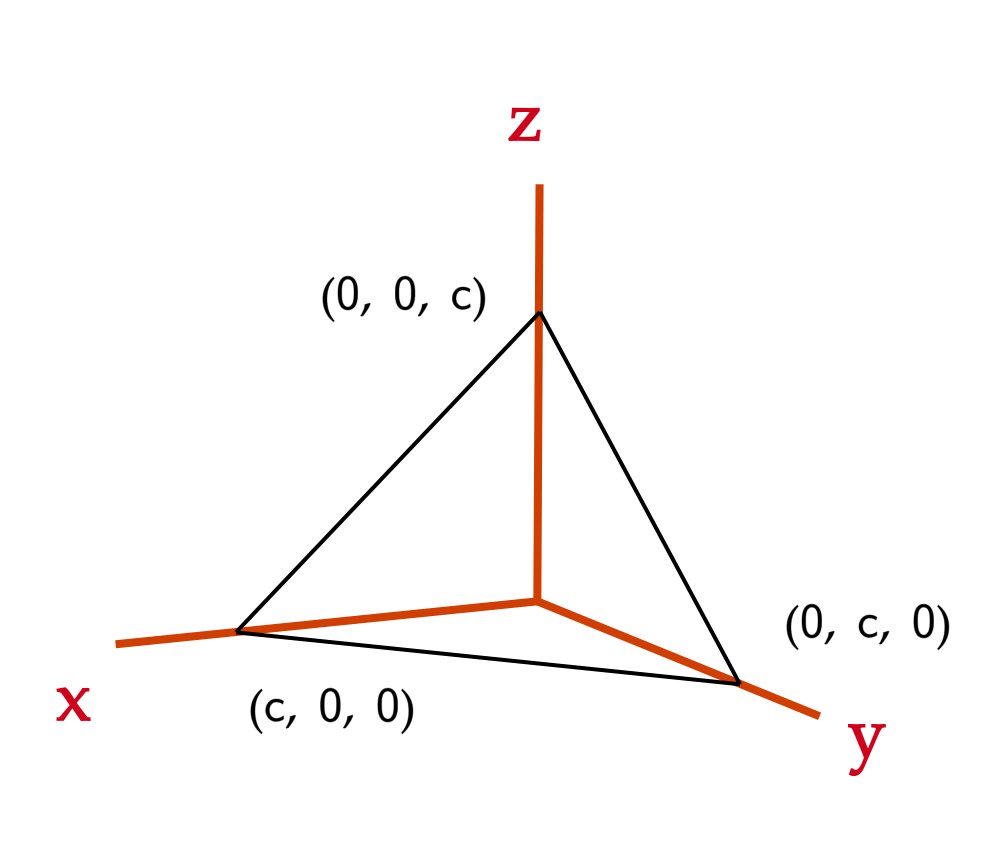
\includegraphics[width=0.8\linewidth]{figures/wk-1/fig-13b.png}
    \end{center}
\end{marginfigure}

\begin{rmk}
    We will briefly review the six \textbf{quadratic surfaces}. These are,
    \begin{enumerate}
        \item The \textbf{ellipsoid}, which is called a sphere when $a = b = c$
        \[\frac{x^2}{a^2}+\frac{y^2}{b^2}+\frac{z^2}{c^2}=1\]
        \item The \textbf{elliptic paraboloid}, which is along the $z$-axis,
        \[\frac{z}{c}=\frac{x^2}{a^2}+\frac{y^2}{b^2}\]
        \item The \textbf{hyperbolic paraboloid},
        \[\frac{z}{c}=\frac{x^2}{a^2}-\frac{y^2}{b^2}\]
        \item The \textbf{cone},
        \[\frac{z^2}{c^2}=\frac{x^2}{a^2}+\frac{y^2}{b^2}\]
        \item The \textbf{hyperboloid of one sheet}, with sheets along $z$,
        \[\frac{x^2}{a^2}+\frac{y^2}{b^2}-\frac{z^2}{c^2}=1\]
        \item The \textbf{hyperboloid of two sheets}, with sheets along $z$,
        \[-\frac{x^2}{a^2}-\frac{y^2}{b^2}+\frac{z^2}{c^2}=1\]
    \end{enumerate}
\end{rmk}

\begin{ex}{Quadratic Surfaces}{label}
    The function $f: \R^3 \rightarrow \R$ defined by
\[f(x, y, z) = x^2 + y^2 + z^2\]
has range$(f) = (\infty, \infty)$ and,
\[f^{-1}(\{c\}) = 0 \text{ and } f^{-1}(\{c\}) \text{ is a sphere for } c > 0\]
If we had instead considered the function,
\[f(x, y, z)=x^2-y^2+z^2\]
then we would have had that,
\[
f^{-1}(\{c\}) \text{ is a } \begin{cases}
                \text{Hyperboloid of Two Sheets} & \text{ for } c < 0 \\
                \text{Circular Cone} & \text{ for } c = 0 \\
                \text{Hyperboloid of One Sheet} & \text{ for } c > 0 \\
                \end{cases}
\]
\end{ex}

\section{Limits and Continuity}
\subsection{Limits of Functions}
\begin{defn}[Open Disk]
     Let $\mathbf{x} \in \R^n$. Given $r > 0$,
     \[D_r(\mathbf{x}_0) := \{\mathbf{x} \in \R^n \mid \|\mathbf{x} - \mathbf{x}_0\| < r\}\]
     is the \textbf{open ball} of radius $r$ centered at $\mathbf{x}$.
\end{defn}

\begin{defn}[Open Subset]
     A subset $U \subset \R^n$ is \textbf{open} if,
     \[\exists r > 0 \text{ such that } D_r(\mathbf{x}_0) \subseteq U \text{ for all } \mathbf{x}_0 \in U\]
\end{defn}

\begin{prop}
    $D_r(\mathbf{x}_0)$ is \textbf{open} according to the preceding definition.
\end{prop}

\begin{proof}
    Let $\mathbf{x}_0$ be arbitrary. We need to show that there exists $s > 0$ such that $D_s(\mathbf{x}_0) \subseteq D_r(\mathbf{x}_0)$. Choose $s := r - \|\mathbf{x} - \mathbf{x}_0\|$. Now,
    \[\|\mathbf{y} - \mathbf{x}_0\| = \|\mathbf{y} - \mathbf{x} + \mathbf{x} - \mathbf{x}_0\| \leq \|\mathbf{y}-\mathbf{x}\|+\|\mathbf{x}-\mathbf{x}_0\| < s + \|\mathbf{x}-\mathbf{x}_0\|\]
    since $\mathbf{y} \in D_s(\mathbf{x})$. By our choice of $s$, it follows that,
    \[\|\mathbf{y} - \mathbf{x}_0\| < r\]
    and consequently $D_r(\mathbf{x}_0)$ is \textbf{open}.
\end{proof}

\begin{marginfigure}
    Choosing $s$ to prove that $D_r(\mathbf{x}_0)$ is open.
    \begin{center}
       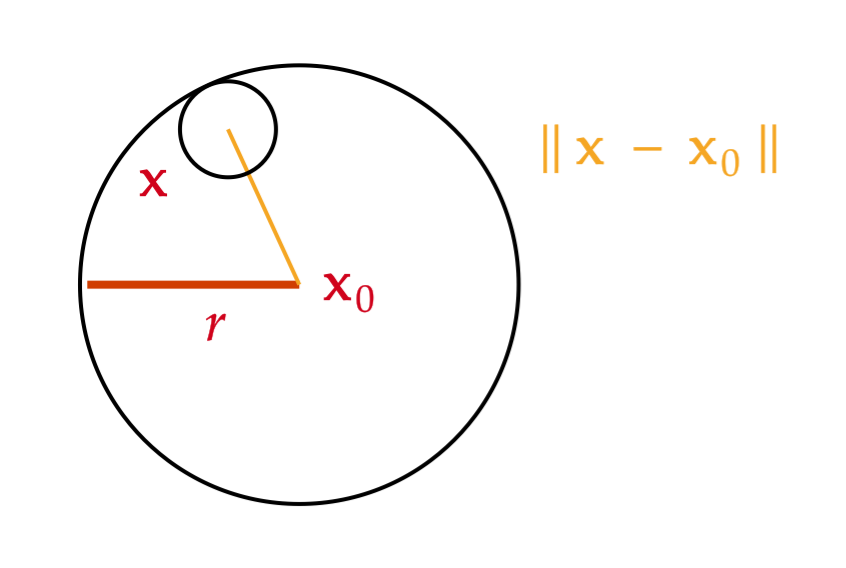
\includegraphics[width=\textwidth]{figures/wk-1/fig-17.png}
    \end{center}
\end{marginfigure}

\begin{marginfigure}
    We say that a \textbf{neighborhood} of $\mathbf{x} \in \R^n$ is an open set $U$ such that $\mathbf{x} \in U$.
\end{marginfigure}

\begin{defn}[Boundary Point]
     We call $\mathbf{x} \in \R^n$ a \textbf{boundary point} of an open set $A$ if every neighborhood of $\mathbf{x}$ contains a point in $A$ and a point in $A^c$. We write $\partial A$ for the set of boundary points of $A$.
\end{defn}

\begin{cor}
    $\partial D_r(\mathbf{x}_0) = \{\mathbf{x} \mid \|\mathbf{x} - \mathbf{x}_0\| = r\}$
\end{cor}

\begin{defn}[Limit of a Function]
    Let $f: A \subseteq R^n \rightarrow \R^m$ be a function defined on an open subset $A$ of $\R^n$. Let $\mathbf{x}_0 \in A \cup \partial A$. Then,
    \begin{enumerate}
        \item \sloppy $f$ is eventually in $N$ as $\mathbf{x}$ approaches $\mathbf{x}_0$ if $\exists U$, a neighborhood of $\mathbf{x}_0$, such that if $\mathbf{x} \neq \mathbf{x}_0$ and $\mathbf{x} \in A \cap U$, then $f(\mathbf{x}) \in N$
        \item $f(\mathbf{x})$ approaches $\mathbf{b}$ as $\mathbf{x}$ approaches $\mathbf{x}_0$ if, given any neighborhood $N$ of $\mathbf{b}$, $f$ is eventually in $N$ as $\mathbf{x}$ approaches $\mathbf{x}_0$ 
    \end{enumerate}
    where $\mathbf{b} \in \text{range}(f) \subseteq \R^m$. In either case, we write,
    \[\lim_{\mathbf{x} \rightarrow \mathbf{x}_0} f(\mathbf{x}) = \mathbf{b}\]
\end{defn}

\begin{center}
   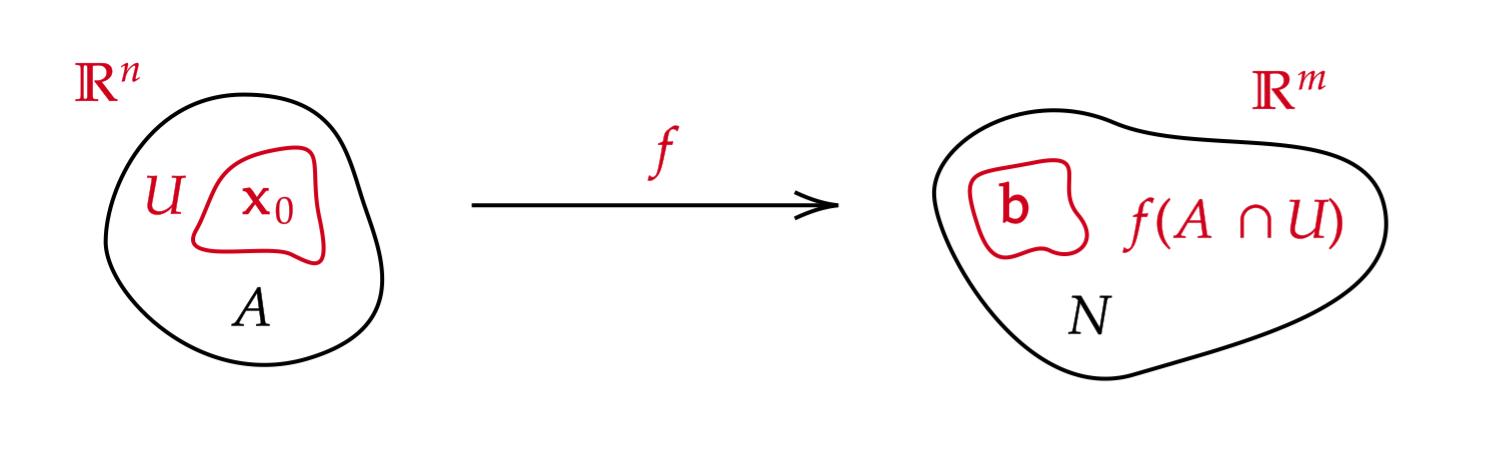
\includegraphics[width=0.8\textwidth]{figures/wk-1/fig-19.png}
\end{center}
    
\begin{marginfigure}
    Example of a boundary point $x$.
    \begin{center}
       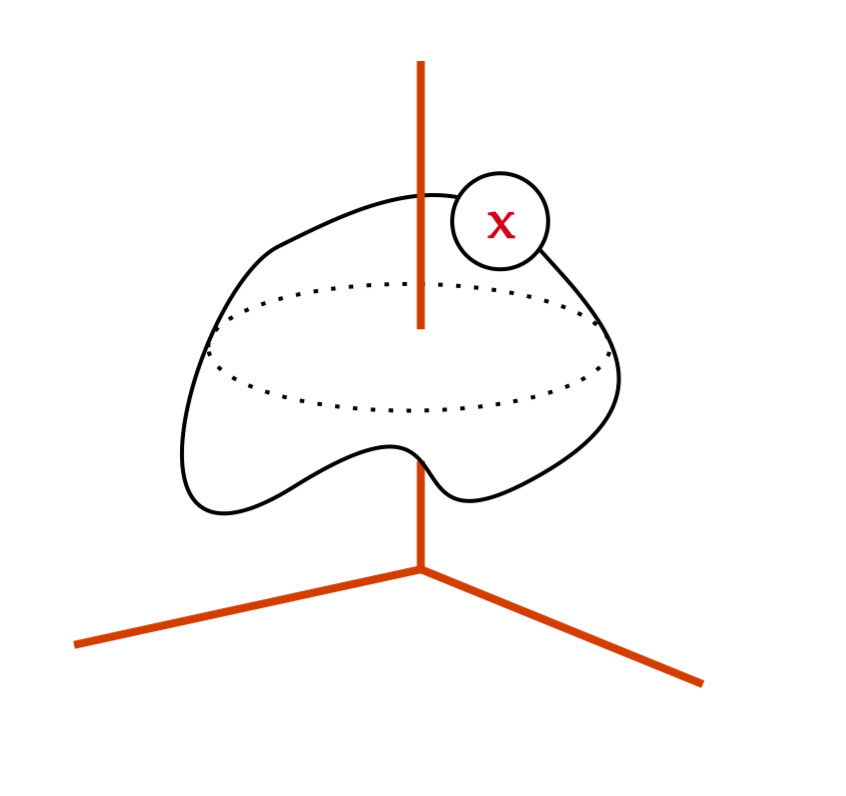
\includegraphics[width=0.8\textwidth]{figures/wk-1/fig-18.png}
\end{center}
\end{marginfigure}

\noindent The following are properties of limits of functions,
\begin{rmk}[Uniqueness of Limits]
Suppose that,
\begin{align*}
    &\lim_{\mathbf{x} \rightarrow \mathbf{x}_0} f(\mathbf{x}) = \mathbf{b}_1 \\
    &\lim_{\mathbf{x} \rightarrow \mathbf{x}_0} f(\mathbf{x}) = \mathbf{b}_2
\end{align*}
Then $\mathbf{b}_1 = \mathbf{b}_2$. That is, if $f$ has a limit at $\mathbf{x}_0$, then that limit is unique.
\end{rmk}

\begin{rmk}[Limit Properties]
Suppose that $A \subset \mathbb{R}^n$, $\mathbf{x}_0 \in A \cup \partial A$, and $f$ and $g$ are functions on $A$ taking values in $\R^m$. If we have that,
\[
\lim_{\mathbf{x} \rightarrow \mathbf{x}_0} f(x)=\mathbf{b}_1 \quad \text { and } \quad \lim_{\mathbf{x} \rightarrow \mathbf{x}_0} f(\mathbf{x})=\mathbf{b}_2
\]
Then the following properties hold,
\begin{enumerate}
    \item $\lim_{\mathbf{x} \rightarrow \mathbf{x}_0} c f(x)= c\mathbf{b}_1$ for $c \in \R$
    \item $\lim_{\mathbf{x} \rightarrow \mathbf{x}_0} (f(x) + g(x)) = \mathbf{b}_1 + \mathbf{b}_2$
    \item If $m = 1$, then $\lim_{\mathbf{x} \rightarrow \mathbf{x}_0} f(x) \cdot g(x) = \mathbf{b}_1 \cdot \mathbf{b}_2$
    \item If $m = 1$ and $f(x) \neq 0$ $ \forall x \in A$, then $\lim_{\mathbf{x} \rightarrow \mathbf{x}_0} 1 / f(x) = 1 / \mathbf{b}_1$ 
\end{enumerate}
\end{rmk}

\subsection{Continuity}
\begin{defn}[Continuity]
    A function $f: A \subseteq \R^n \rightarrow \R^m$ is called \textbf{continuous} on $A$ if it is \textbf{continuous at every point} $\mathbf{x_0} \in A$.
\end{defn}

\begin{thm}[Continuity of Compositions]
    Let $f: A \subseteq \R^n \rightarrow \R^m$ and $g: B \subseteq \R^m \rightarrow \R^l$ be two functions with $f(A) \subseteq B$. If $f$ is continuous at $\mathbf{x}_0$ and  $g$ is continuous at $f(\mathbf{x}_0)$, then the composition,
    \[g \circ f : A \subseteq \R^n \rightarrow \R^l\]
    is continuous at $\mathbf{x}_0$.
\end{thm}

\begin{center}
       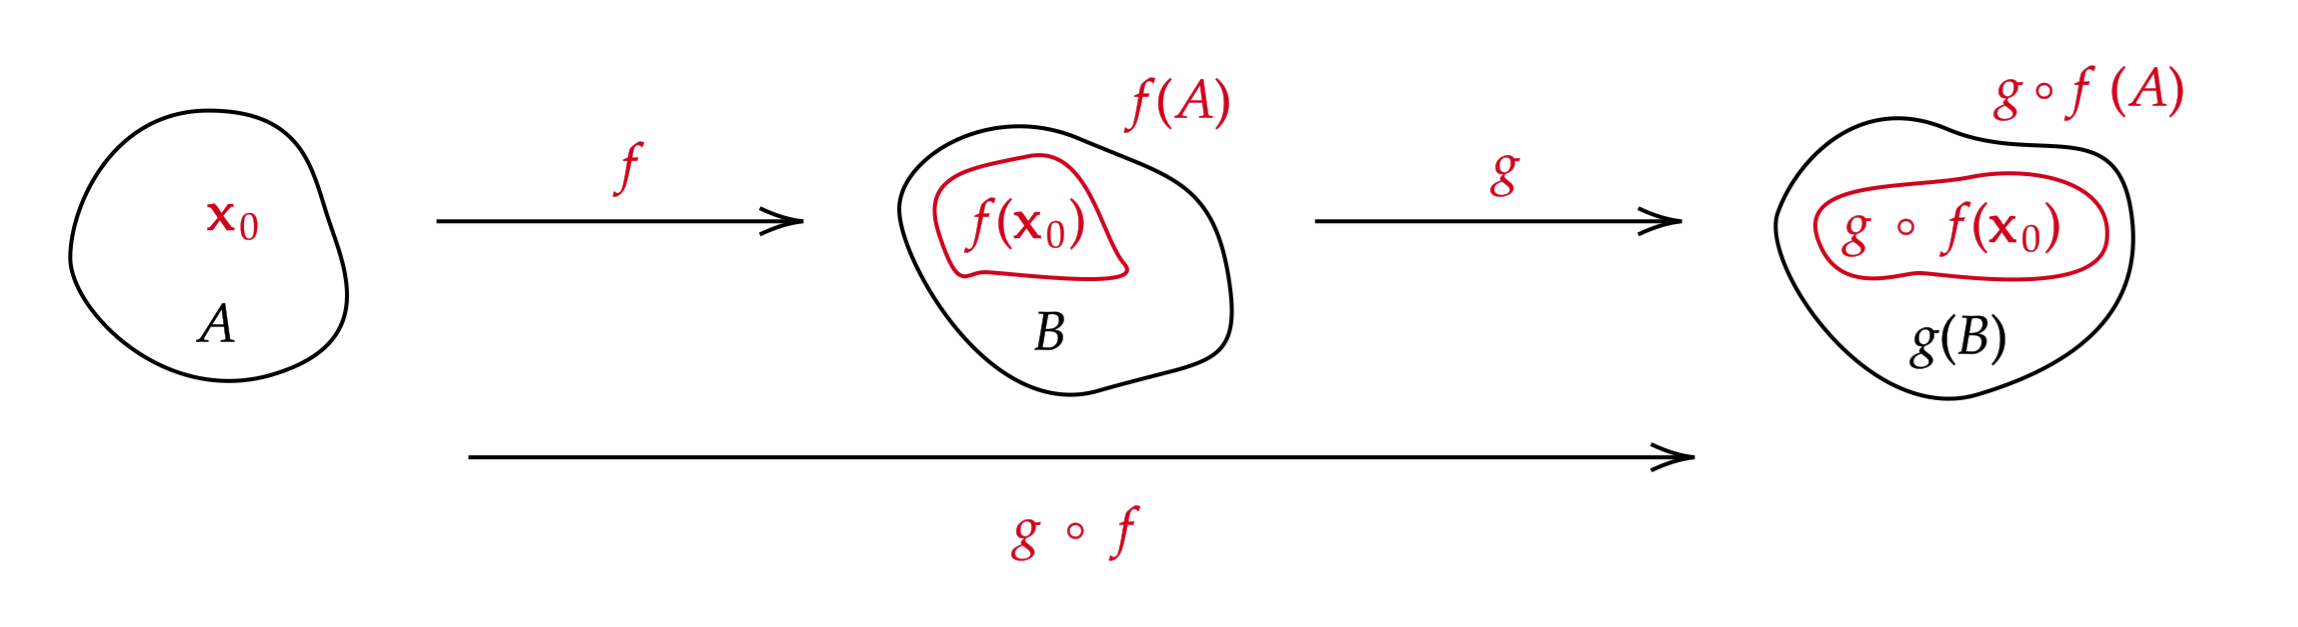
\includegraphics[width=0.8\textwidth]{figures/wk-1/fig-20.png}
\end{center}

\noindent We want to formulate the property of continuity precisely.

\begin{thm}
    Consider $f: A \subseteq \R^n \rightarrow \R^m$. Let $\mathbf{x}_0 \in A$ or $\mathbf{x}_0 \cup \partial A$.
    \begin{enumerate}
        \item If $\forall \epsilon > 0$, $\exists \delta(\epsilon) > 0$ such that $\|\mathbf{x} - \mathbf{x}_0\| < \delta$ implies that,
        \[\|f(\mathbf{x}) - \mathbf{b}\| < \epsilon\]
        then we have that  $\lim_{\mathbf{x} \rightarrow \mathbf{x_0}} f(\mathbf{x})= \mathbf{b}$
        \item $f$ is continuous at $\mathbf{x}_0 \in A$ if and only if  $\lim_{\mathbf{x} \rightarrow \mathbf{x_0}} f(\mathbf{x})= f(\mathbf{x_0})$
        
    \end{enumerate}
\end{thm}

\begin{ex}{Continuity via Composition}{label}
    We can prove that the function \text{$f: \R^3 \rightarrow \R$} defined by,
    \[f(x, y, z) = e^{-(x^2 + y^2 + z^2)}\]
    is continuous for all $\mathbf{x} \in \R^3$ using continuity of compositions:
    \begin{enumerate}
        \item $f_1(t) = e^{-t}$ is continuous for all $t \in \R$
        \item $f_2(x, y, z) = -(x^2 + y^2 + z^2)$ is continuous for all $\mathbf{t} \in \R^3$
    \end{enumerate}
    Thus, $f = f_1 \circ f_2 = e^{-(x^2 + y^2 + z^2)}$ is continuous for all $\mathbf{x} \in \R^3$.
\end{ex}

\begin{marginfigure}
    The graph of $f: \R^2 \rightarrow \R$ defined by,
    \[f(x, y) = \frac{4x^2y}{x^2 + y^2}\]
    \begin{center}
       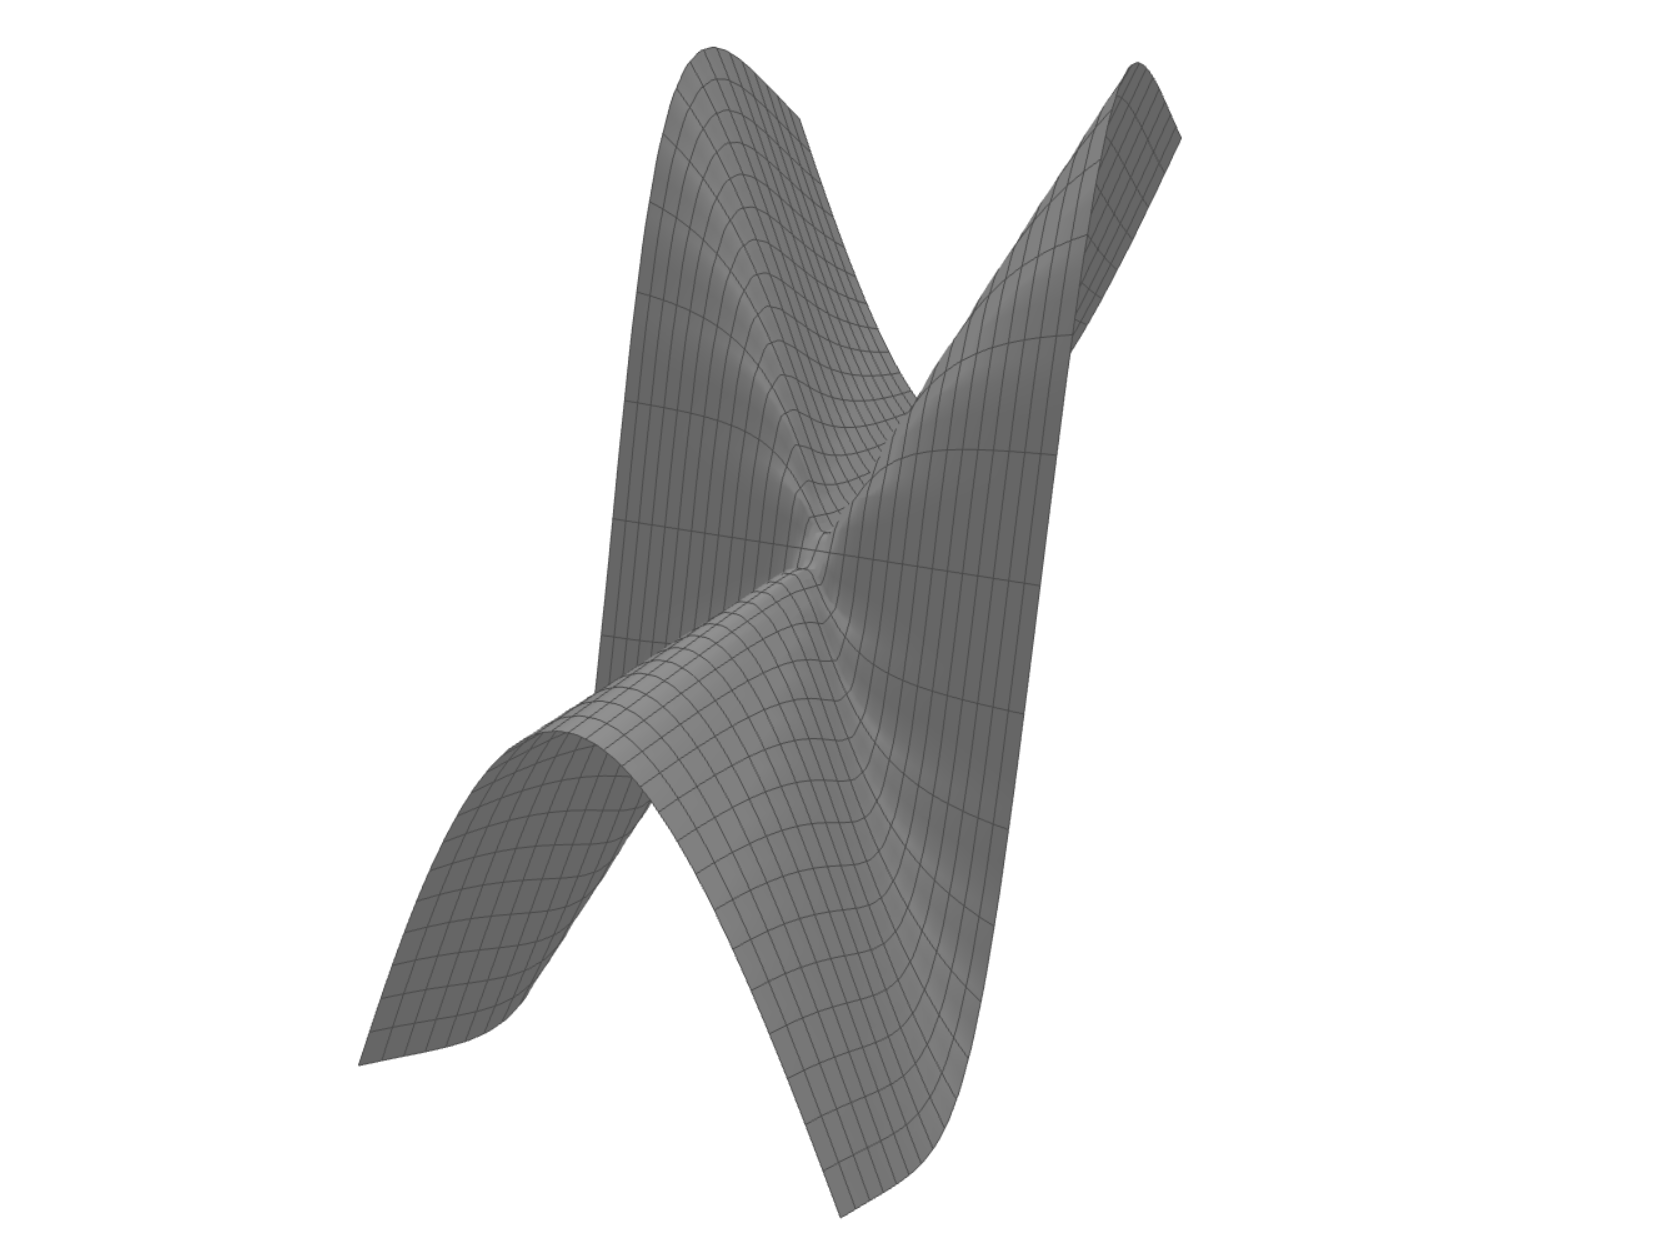
\includegraphics[width=0.7\textwidth]{figures/wk-1/fig-22.png}
    \end{center}
    
    \LineBreak

    The graph of $f: \R^2 \rightarrow \R$ defined by,
    \[f(x, y) = \frac{x^2y^2}{x^2 + y^2}\]
    \begin{center}
        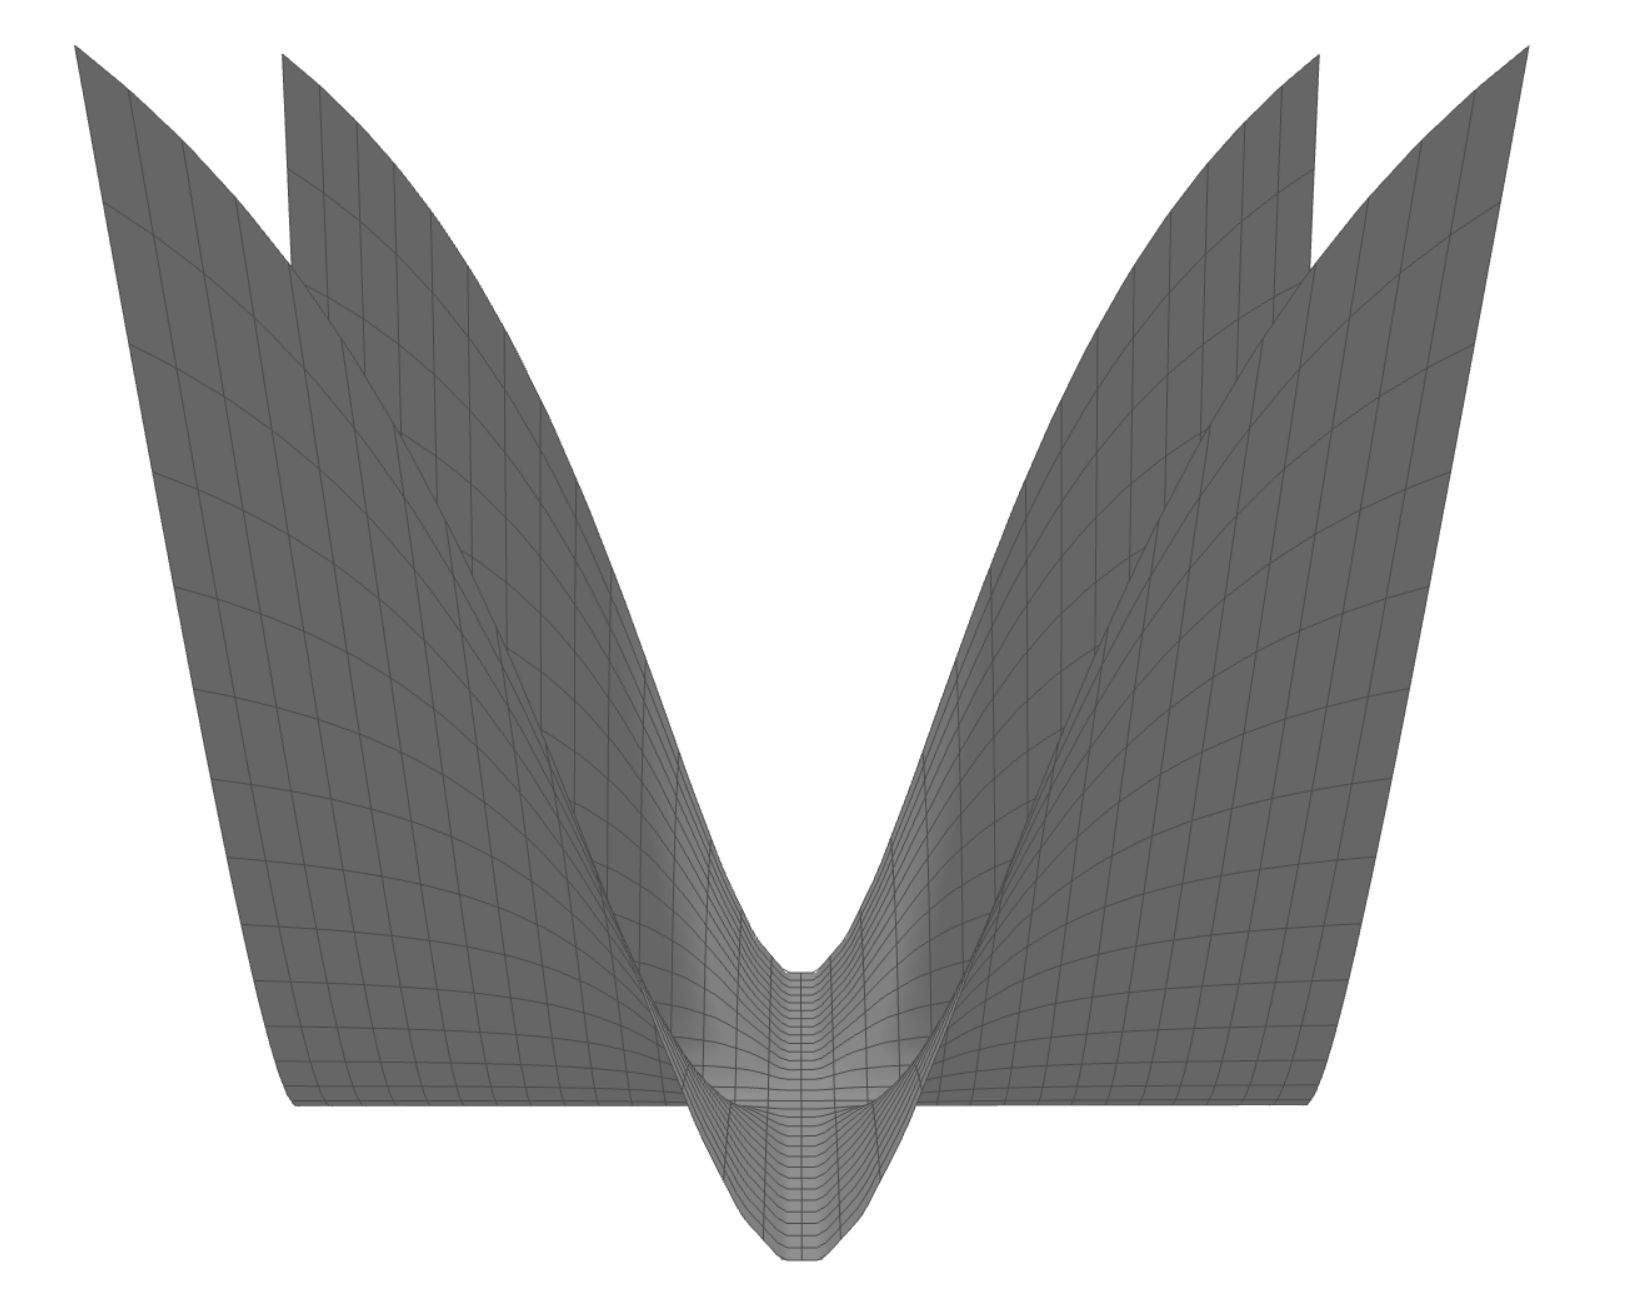
\includegraphics[width=0.6\textwidth]{figures/wk-1/fig-23.png}
    \end{center}
    
\end{marginfigure}

\begin{ex}{$f(x, y) = x + y$}{label}
    We will prove that the function,
    \begin{align*}
        &f: \R^2 \rightarrow \R \\
        &f(x, y) = x + y
    \end{align*}
    is continuous. Let \text{$\epsilon > 0$} be arbitrary and define \text{$\delta(\epsilon) := \frac{\epsilon}{2}$}. Suppose that $\|\mathbf{x} - \mathbf{x}_0\| < \delta$. Then,
    \[|x + y - (x_0 + y_0)| \leq \underbrace{|x - x_0 |}_{< \delta(\epsilon)} + \underbrace{|y - y_0|}_{< \delta(\epsilon)} < \frac{\epsilon}{2} + \frac{\epsilon}{2} = \epsilon\]
    since,
    \[\delta > \|\mathbf{x} - \mathbf{x}_0\| = \sqrt{(x - x_0)^2 + (y - y_0)^2} \geq \sqrt{(x - x_0)^2} = |x - x_0|\]
    and
    \[\delta > \|\mathbf{x} - \mathbf{x}_0\| = \sqrt{(x - x_0)^2 + (y - y_0)^2} \geq \sqrt{(x - x_0)^2} = |y - y_0|\]
\end{ex}

\begin{ex}{$f(x, y) = 4x^2y / x^2 + y^2$}{label}
    We will prove that the function,
    \begin{align*}
        &f: \R^2 \rightarrow \R \\
        &f(x, y) = \frac{4x^2y}{x^2 + y^2}
    \end{align*}
    approaches $\mathbf{0}$ as \text{$(x,y) \rightarrow (0,0)$}. Let \text{$\epsilon > 0$} be arbitrary and define \text{$\delta(\epsilon) = \frac{\epsilon}{4}$}. Suppose that $\|\mathbf{x} - \mathbf{0}\| = \|\mathbf{x}\| < \delta$.
    \[\left|\frac{4x^2y}{x^2 + y^2}\right| \leq \left|\frac{4x^2y}{x^2}\right| = 4 |y| \leq 4\|\mathbf{x}\| < \epsilon\]
\end{ex}

\begin{ex}{$f(x, y) = x^2y^2 / x^2 + y^2$}{label}
    We will prove that the function,
    \begin{align*}
        &f: \R^2 \rightarrow \R \\
        &f(x, y) = \frac{x^2y^2}{x^2 + y^2}
    \end{align*}
    approaches $\mathbf{0}$ as \text{$(x,y) \rightarrow (0,0)$}. Let \text{$\epsilon > 0$} be arbitrary and define $\delta(\epsilon) = \sqrt{\epsilon}$. Suppose that $\|\mathbf{x} - \mathbf{0}\| = \|\mathbf{x}\| < \delta$.
    \[\left|\frac{x^2y^2}{x^2 + y^2}\right| = |x|^2 \cdot \underbrace{\left|\frac{y^2}{x^2 + y^2}\right|}_{< 1} \leq |x|^2 \leq \|\mathbf{x}\|^2 < \epsilon\]
\end{ex}